% !TeX program = pdfLaTeX
\documentclass[smallextended]{svjour3}       % onecolumn (second format)
%\documentclass[twocolumn]{svjour3}          % twocolumn
%
\smartqed  % flush right qed marks, e.g. at end of proof
%
\usepackage{amsmath}
\usepackage{graphicx}
\usepackage[utf8]{inputenc}

\usepackage[hyphens]{url} % not crucial - just used below for the URL
\usepackage{hyperref}
\providecommand{\tightlist}{%
  \setlength{\itemsep}{0pt}\setlength{\parskip}{0pt}}

%
% \usepackage{mathptmx}      % use Times fonts if available on your TeX system
%
% insert here the call for the packages your document requires
%\usepackage{latexsym}
% etc.
%
% please place your own definitions here and don't use \def but
% \newcommand{}{}
%
% Insert the name of "your journal" with
% \journalname{myjournal}
%

%% load any required packages here
\usepackage{amsfonts} \usepackage{algorithm}
\usepackage[noend]{algpseudocode}
\makeatletter \def\BState{\State\hskip-\ALG@thistlm}
\makeatother \usepackage{booktabs} \usepackage{longtable}
\usepackage{array} \usepackage{multirow} \usepackage[table]{xcolor}
\usepackage{wrapfig} \usepackage{float} \usepackage{colortbl}
\usepackage{pdflscape} \usepackage{tabu} \usepackage{threeparttable}
\usepackage{threeparttablex} \usepackage[normalem]{ulem}
\usepackage{makecell}
\usepackage{float}



\begin{document}

\title{Metric space change point detection \thanks{Grants or other notes about the article that should go on the front page
should be placed here. General acknowledgments should be placed at the
end of the article.} }


    \titlerunning{Metric change point detection}

\author{  David Letscher \and  Darrin Speegle }


\institute{
        David Letscher \at
     Department of Computer Science, Saint Louis University \\
     \email{\href{mailto:david.letscher@slu.edu}{\nolinkurl{david.letscher@slu.edu}}}  %  \\
%             \emph{Present address:} of F. Author  %  if needed
    \and
        Darrin Speegle \at
     Department of Mathematics and Statistics, Saint Louis University \\
     \email{\href{mailto:darrin.speegle@slu.edu}{\nolinkurl{darrin.speegle@slu.edu}}}  %  \\
%             \emph{Present address:} of F. Author  %  if needed
    }

\date{Received: date / Accepted: date}
% The correct dates will be entered by the editor


\maketitle

\begin{abstract}
Let \((x_t)_{t = 1}^N\) be a time series with values in a metric space
\(X\), which is locally isometric to Euclidean space. A transformation
of the data is proposed which produces a multi-dimensional time series
of real numbers. If the original sequence of data points has a single
change point in mean at time \(t_0\), then with high probability the
transformed data will also have a single change point in mean at time
\(t_0\). Applications to time series of persistence diagrams are
considered.
\\
\keywords{
        change point detection \and
        metric space \and
        persistence \and
        tda }

    \subclass{
                    MSC code 1 \and
                    MSC code 2 }

\end{abstract}


\def\spacingset#1{\renewcommand{\baselinestretch}%
{#1}\small\normalsize} \spacingset{1}


\section{Introduction}\label{intro}

A simple change point detection problem is the following: suppose that
\((x_t)_{t = 1}^{t_0}\) are iid Gaussian random variables with mean
\(\mu_0\) and variance \(\sigma\), and \((x_t)_{t = t_0 + 1}^N\) are iid
Gaussian with mean \(\mu_1\) and variance \(\sigma\). The goal is to
determine whether \(\mu_0 = \mu_1\), and if not, then what the value of
\(t_0\) is.

\begin{figure}[h!]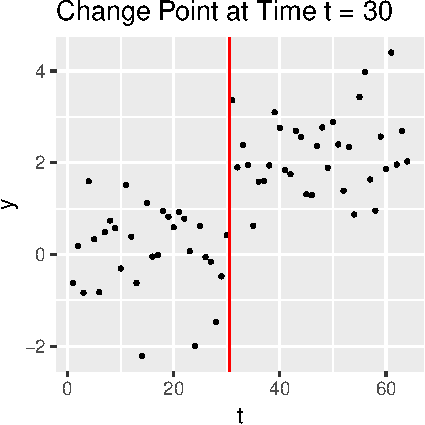
\includegraphics{springer_template_files/figure-latex/chunk_1-1} \caption{Simple change point}\label{fig:1}\end{figure}

More general problems include having multiple change points, noise that
is not Gaussian, underlying signals that are not constant, and
multi-dimensional signals.

In this paper, we consider the following set-up. Let \(X\) be a metric
space. Supose that \(f:[0,1]\to X\) is a piecewise continuous function
with at most one discontinuity. Let \((a_t)_{t = 1}^N\) be an increasing
sequence of numbers in \((0, 1)\) and \(\delta > 0\) such that for each
\(y\in [0,1]\), \(B_\delta(f(y))\) is isometric to Euclidean space. Let
\(x_t = f(a_t) + \epsilon_t\), where \(\epsilon_t\) is a uniformly
distributed random variable on \(B_\delta(f(a_t))\). Our problem is to
determine whether there exists a point of discontinuity \(y_0\) of \(f\)
and a \(k < N\) such that the discontinuity is contained between \(a_k\)
and \(a_{k +1}\). If there does exist such a \(k\), then we should also
estimate it.

Our motivation is that we wish to find change points in time series of
\textbf{persistence diagrams}. Persistence diagrams are a way of
measuring the topological structure of a point cloud in Euclidean space.
More here.

\section{Metric space change point detection algorithm}\label{sec:1}

With the notation as set up in Section \ref{intro}, we proceed to
describe the algorithm for change point detection for time series data
in metric spaces. The main step is transforming the data into a
multi-dimensional time series of real numbers in such a way as to
preserve the change point, see Algorithm \ref{euclid}.

\begin{algorithm}\label{algo:1}
\caption{Transform to Real}\label{euclid}
\begin{algorithmic}[1]
\Procedure{MyProcedure}{}
\State $\textit{time\_length} \gets \text{length of }\textit{time\_series}$
\State $i \gets 1$
\While {$\textit{i < time\_length}$}
\State $\textit{A, B} \gets \text{sample(N, 2, replace = FALSE)}$
\For {$j \gets 1:time\_length$}
\State $\textit{dists[j,i]} \gets (d(A, x_j)^2 - d(B, x_j)^2)/d(A, B)$
\EndFor
\State $\textit{i++}$
\EndWhile
\EndProcedure
\end{algorithmic}
\end{algorithm}

Once the metric space valued time series is transformed into a
multi-dimensional real valued time series, standard techniques can be
used to determine if and where a change point occurs. In this paper, we
use the \texttt{cpbaywave} package, as it finds change points in high
dimensional, smooth data with a single discontinuity. We illustrate the
usage with some examples.

\begin{example}\label{ex:1} Suppose that the time series lives in
\(\mathbb {R}^M\) for some \(M\). For example, we could have a time
series of length 128 in 100 dimensional data, with a change point at
time \(t = 80\). We consider two examples in this case; in both
examples, the data has mean zero in all dimensions until time 80. In the
first case, it has mean 0.1 in all dimensions from dimension 81 through
128 and in the second case it has mean 1 and all dimensions from
dimension 81 through 128. In all cases, the standard deviation is 1.

As shown in Figure \ref{fig:2}, in the case that the mean increases by 0.1, the algorithm is not able to
locate the change point, and incorrectly determines that there is no change. We note that \texttt{cpbaywave} was also unable to detect the change point when using the untransformed data.

\begin{figure}[h!]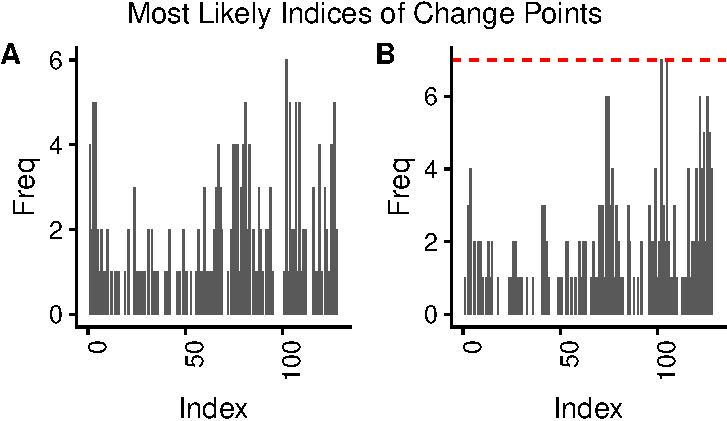
\includegraphics{springer_template_files/figure-latex/chunk_3-1}
\caption{Plot A is from raw data, and plot B is from transformed data. In neither case is the change point detected}
 \label{fig:2}\end{figure}

However, as shown in Figure \ref{fig:3} and Table \ref{tab:chunk_4_5}, the algorithm is able to correctly identify the change point of $t = 80$ when the mean increases by 1. We note that \texttt{cpbaywave} was also able to detect the change point using the untransformed data.


\begin{figure}[H]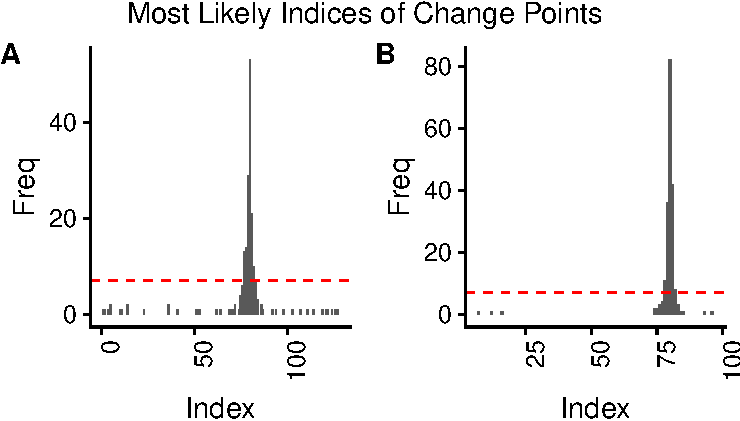
\includegraphics{springer_template_files/figure-latex/chunk_4_5-1} 
\caption{Plot A is from raw data, and plot B is from transformed data. In both cases, the change point is detected.}
\label{fig:3}\end{figure}

\goodbreak
\begin{longtable}[t]{lrll}
\caption{\label{tab:chunk_4_5}Indices which are significant, together with their frequency. True change point at t = 80.}\\
\toprule
\multicolumn{2}{c}{Raw Data} & \multicolumn{2}{c}{Transformed Data} \\
\cmidrule(l{2pt}r{2pt}){1-2} \cmidrule(l{2pt}r{2pt}){3-4}
Index & Freq & Index & Freq\\
\midrule
77 & 13 & 78 & 11\\
78 & 14 & 79 & 36\\
79 & 29 & 80 & 82\\
80 & 53 & 81 & 42\\
81 & 21 & 82 & 8\\
82 & 10 &  & \\
\bottomrule
\end{longtable}

This picture gives a typical strong indication that there is a change
point at or near time \(t = 80\), which we know is the correct value.

We note here that the \texttt{cpbaywave} algorithm also fails to detect
a change point in the first example when using the untransformed data.
\end{example}

\begin{example} Next, we consider a change in mean from $\mu = 0$ to $\mu = 1$ at time $t = 80$, as above, but we imagine the time series living in \(\ell_{4}^{100}\) rather than in \(\ell_{2}^{100}\). Since $\ell_{4}^{100}$ is not locally Euclidean, this example is testing the robustness of our algorithm to our assumptions. As can be seen in Figure \ref{fig:4} and Table \ref{tab:chunk_5_75}, the change point is detected in the raw data (which we had already seen in Example \ref{ex:1}) as well as the transormed data. Thus, our algorithm appears to have some robustness to non-Euclidean metric spaces.

\begin{figure}[H]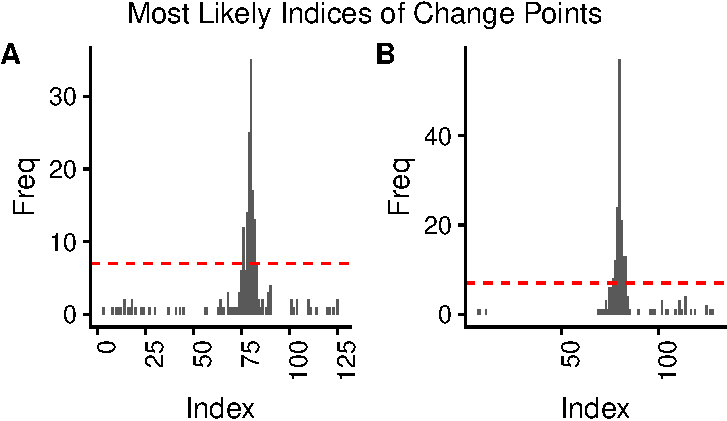
\includegraphics{springer_template_files/figure-latex/chunk_5_5-1} 
\caption{Plot A is from raw data, and plot B is from transformed data, assuming that the data lives in $\ell^4$. In both cases, the change point is detected.}
\label{fig:4}\end{figure}

\begin{longtable}[t]{lllr}
\caption{\label{tab:chunk_5_75}Indices which are significant, together with their frequency.}\\
\toprule
\multicolumn{2}{c}{Raw Data} & \multicolumn{2}{c}{Transformed Data} \\
\cmidrule(l{2pt}r{2pt}){1-2} \cmidrule(l{2pt}r{2pt}){3-4}
Index & Freq & Index & Freq\\
\midrule
76 & 12 & 77 & 8\\
78 & 14 & 78 & 12\\
79 & 25 & 79 & 24\\
80 & 35 & 80 & 57\\
81 & 17 & 81 & 21\\
\addlinespace
82 & 13 & 82 & 13\\
 &  & 83 & 13\\
\bottomrule
\end{longtable}
\end{example}

\section{Change points in persistence diagrams}\label{sec:2}

The space of persistence diagrams is not locally isometric to Euclidean
space. However, it does seem to be closer to being isometric to
Euclidean space than \(\ell^4\) is. We apply our algorithm now for time
series of persistence diagrams. First, we apply it to simulated data,
then to data in the wild of various types.

\begin{example}\label{ex:3} Our first example is of two time series of simulated point clouds with strong topological properties. For the first time series, we start with a single circle, sampled randomly with normal jitter, and then at time \(t = 80\), we add a second point cloud sampled from a disjoint circle with normal jitter added. Any good change point detection algorithm based on persistence diagrams should be able to find such a change. Figure \ref{fig:5} shows time samples before and after the change point.

\begin{figure}[H]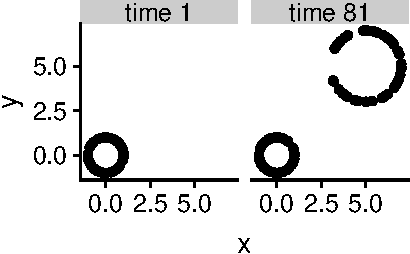
\includegraphics{springer_template_files/figure-latex/chunk_6-1}
\caption{Point clouds before and after the change point, where a second circle is added.}
 \label{fig:5}\end{figure}

The change point detection algorithm easily detects the change, as seen in Figure \ref{fig:6}. 

\begin{figure}[H]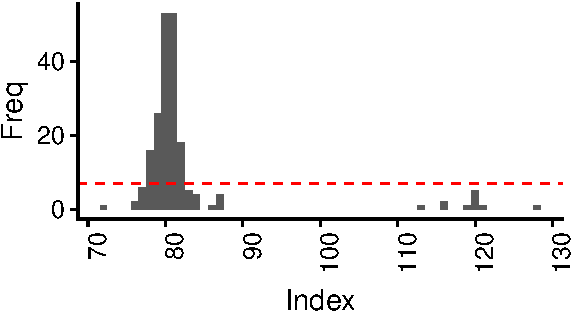
\includegraphics{springer_template_files/figure-latex/unnamed-chunk-1-1} 
\caption{Change point detected when second circle is added at time $t = 80$.}
\label{fig:6}\end{figure}

As seen in Table \ref{tab:unnamed-chunk-2}, times 80 and 81 were the most commonly chosen times for the change point in the bootstrap algorithm, with 78, 79 and 82 also making the cutoff to be significant. 
\begin{longtable}[t]{lr}
\caption{\label{tab:unnamed-chunk-2}Indices which are significant, together with their frequency. True change point at t = 80.}\\
\toprule
Index & Freq\\
\midrule
78 & 16\\
79 & 26\\
80 & 53\\
81 & 53\\
82 & 18\\
\bottomrule
\end{longtable}

Our second example of simulated data is more challenging. We sample from two circles (again with normal jitter) which start out being disjoint, but over time one of the two circles moves so that it intersects the other circle. From a topological
point of view, there are two potential change points. The first change
point is when there are no longer two connected components, but rather
one. The second change is when there are three loops rather than two.
The algorithm currently under discussion only finds a single change
point; how many and which dimensions are included in the persistence
diagram and distance calculation will determine which change is
detected.

Figure \ref{fig:7} shows the point clouds at three time points, which illustrate the three different (topological) states that the point couds may have. See also \href{http://stat.slu.edu/~speegle/Circles2.gif}{here} for a .gif showing the entire time series.

\begin{figure}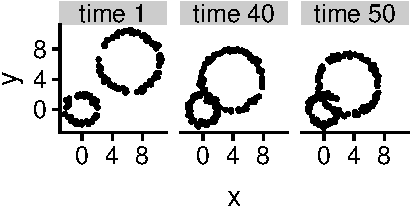
\includegraphics{springer_template_files/figure-latex/chunk_7-1} 
\caption{Circles move through each other. Topological change point not clearly defined.}
\label{fig:7}\end{figure}

In Figure \ref{fig:8}, we see that the change point detection algorithm detects approximately
when three distinct loops become show in the time series. Note that in this case, we only
used 1-dimensional homology in our distance calculation, so our algorithm would not be able to detect changes
in clusters. 

\begin{figure}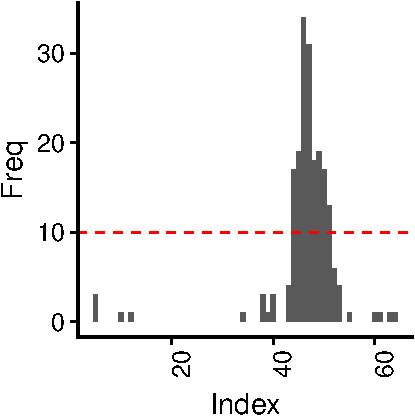
\includegraphics{springer_template_files/figure-latex/chunk_7_5-1} 
\caption{When two circles move through each other, a topological change is detected when the third loop becomes prominent, at or about time $t = 46$.}
\label{fig:8}\end{figure}

Finally, we see in Table \ref{tab:unnamed-chunk-3} that 8 different indices are significant via the bootstrap, with the most likely candidate being time $t = 46$. 

\begin{longtable}[t]{lr}
\caption{\label{tab:unnamed-chunk-3}Indices which are significant, together with their frequency. True change point ambiguous.}\\
\toprule
Index & Freq\\
\midrule
44 & 17\\
45 & 19\\
46 & 34\\
47 & 31\\
48 & 18\\
\addlinespace
49 & 19\\
50 & 17\\
51 & 13\\
\bottomrule
\end{longtable}
\end{example}

Now, we turn to image data. Our basic algorithm is to take a time series of images, find the edges at each time, sample from the edges at each time to form a time series of point clouds, then follow Algorithm \ref{algo:1}. We illustrate this with two examples. In one example, we look at pictures of Table Mountain over time, and it is not completely clear whether or when there is a change point in the time series. In the other example, we examine pictures of a cell dividing, in which case there is a clear change in (topological) characteristics of the images at the time of cell division. 


\begin{example} 
In our first example, we use data from the Archive of Many Outdoor Scenes. We picked a
camera that was taking pictures of Table Mountain in
South Africa. For each day, we averaged all of the pictures that were
taken on that day. We then used edge detection to extract edges from the
pictures, and we removed the time stamp. Finally, we randomly sampled
points from the detected edges of the pictures to use as our point
cloud. So, the time series consists of randomly sampled points from
edges of the average of all pictures on 64 consecutive days. The
original averaged images are
\href{http://stat.slu.edu/~speegle/Kaapstad.gif}{here} and the sampled
edges are \href{http://stat.slu.edu/~speegle/Slide4.gif}{here}. Note that these time series are longer than length 64; we only used the first 64 images in our algorithm to avoid complications of padding.

In Figure \ref{fig:9}, we see that no change point is detected in the time series, though one of the index 63 did beat the nominal bootstrap line. 

\begin{figure}[H]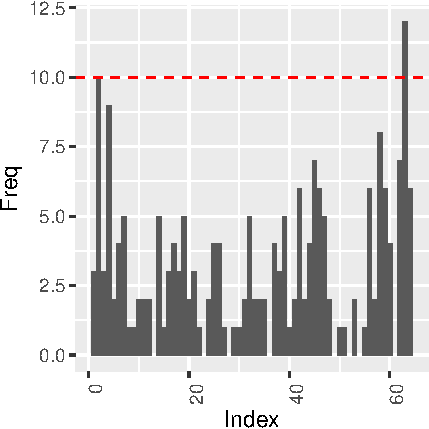
\includegraphics{springer_template_files/figure-latex/chunk_8-1} 
\caption{No significant change point found in the Table Mountain images.}
\label{fig:9}\end{figure}
\end{example}

\begin{example}
In our last example, we have a series of images of a cell, which divides at
about time \(t = 23\). See \href{http://stat.slu.edu/~speegle/cellsRaw.gif}{here} here for the raw data, We again used the
\texttt{cannyEdges} function in the \texttt{imager} R package to detect
the edges of the cells. We then randomly sampled 200 points from the
detected edges at each time stamp to form our time series of point
clouds, see \href{http://stat.slu.edu/~speegle/mycells2.gif}{here} for the results. See Figure \ref{fig:10} for typical pictures before and after the change point. We
then applied Algorithm \ref{algo:1} to detect change points.


\begin{figure}[H]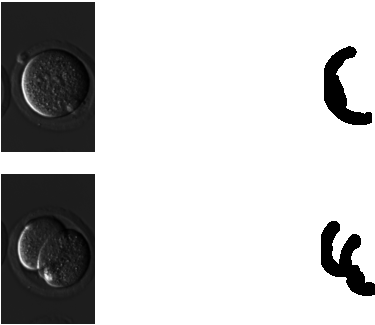
\includegraphics{springer_template_files/figure-latex/chunk_10_5-1} 
\caption{Raw image of cells before and after dividing, together with edge detection.}
\label{fig:10}\end{figure}

In Figure \ref{fig:11}, we see good evidence of a change near the time $t = 23$, which was estimated to be the correct time by the authors. 

\begin{figure}[H]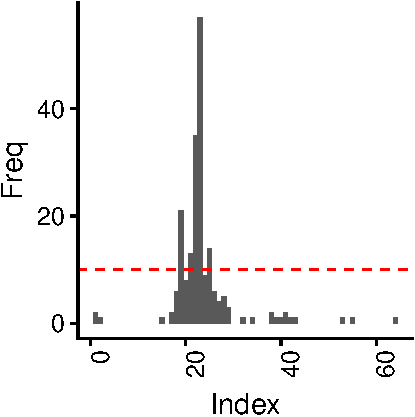
\includegraphics{springer_template_files/figure-latex/chunk_11-1} 
\caption{Detects change at or around time $t = 23$.}
\label{fig:11}\end{figure}

Table \ref{tab:chunk_12} shows the significant indices from the bootstrap. There are more than would be ideal, but the change points do at least tend to cluster around the correct value, indicating that there is something of intereste at or near those points.

\begin{longtable}[t]{lr}
\caption{\label{tab:chunk_12}Indices which are significant, together with their frequency. True change point at time t = 23}\\
\toprule
Index & Freq\\
\midrule
19 & 21\\
21 & 13\\
22 & 35\\
23 & 57\\
25 & 14\\
\bottomrule
\end{longtable}
\end{example}

\section{References}\label{references}

\bibliographystyle{spbasic}
\bibliography{bibliography.bib}

\end{document}
